% Chapter 4 - Implementasi dan Pembahasan
\chapter{IMPLEMENTASI DAN PEMBAHASAN}
\label{chap:implementasi}

\section{Implementasi dan Uji Coba Sistem}

Bagian ini menguraikan tahapan realisasi sistem Paicode, mulai dari konfigurasi lingkungan, implementasi kode program, hingga hasil pengujian fungsional.

\subsection{Lingkungan Implementasi}
Sistem diimplementasikan pada lingkungan sistem operasi Ubuntu dengan spesifikasi konfigurasi seperti tercantum pada Tabel~\ref{tab:konfigurasi}.

\begin{longtable}{@{}p{0.30\textwidth}p{0.64\textwidth}@{}}
  \caption{Konfigurasi Lingkungan Implementasi}\label{tab:konfigurasi}\\
  \toprule
  \textbf{Komponen} & \textbf{Spesifikasi} \\
  \midrule
  \endfirsthead
  \toprule
  \textbf{Komponen} & \textbf{Spesifikasi} \\
  \midrule
  \endhead
  Sistem Operasi & Ubuntu (Linux) \\
  Python & \texttt{\textgreater= 3.10} \\
  Manajer Dependensi & pip dan virtual environment \\
  LLM Provider & Gemini (via \texttt{google-generativeai}) \\
  Antarmuka Terminal & \texttt{rich} (output) dan \texttt{prompt\_toolkit} (input) \\
  Hardware & CPU x86\_64, RAM 8+ GB \\
  \bottomrule
\end{longtable}

Proses instalasi dilakukan menggunakan \texttt{Makefile} yang mengotomasi pembuatan virtual environment dan instalasi dependensi dari berkas \texttt{requirements.txt} dan \texttt{setup.cfg}.

\subsection{Implementasi Fitur Utama}

Implementasi inti Paicode berpusat pada arsitektur \textit{Single-Shot Intelligence} yang terbagi menjadi beberapa modul utama seperti yang telah dirancang pada Bab III.

\subsubsection{Manajemen Konfigurasi dan API Key}
Modul \texttt{config.py} mengelola penyimpanan API key secara aman. Kunci disimpan dalam berkas JSON terenkripsi sederhana (hak akses owner-only) di direktori \texttt{~/.config/pai-code/}. Kunci API ini penting untuk otentikasi dengan layanan Gemini. Perintah yang digunakan untuk mengatur dan memvalidasi konfigurasi kunci API ditunjukkan pada Listing~\ref{lst:config-cmd}.

\begin{lstlisting}[language=bash,caption={Perintah konfigurasi API Key}, label={lst:config-cmd}]
pai config set AIzaSy...  # Mengatur key
pai config validate       # Memvalidasi koneksi ke Gemini
\end{lstlisting}

\subsubsection{Implementasi Agen (Single-Shot Intelligence)}
Agen diimplementasikan dalam \texttt{agent.py}. Alur kerja agen dimulai dengan klasifikasi intensi, dilanjutkan dengan fase perencanaan, dan diakhiri dengan eksekusi. Struktur data JSON yang digunakan untuk merepresentasikan rencana eksekusi agen dapat dilihat pada Listing~\ref{lst:agent-planning}.

\medskip
\lstinputlisting[language=Python, captionpos=b, caption={Cuplikan agent.py (Struktur Planning JSON)}, firstline=640, lastline=660, label={lst:agent-planning}]{../paicode/paicode/agent.py}

Selain format data, agen juga dibekali instruksi sistem (\textit{System Prompt}) yang mendefinisikan persona dan batasan arsitektur \textit{Single-Shot} agar model fokus pada perencanaan yang presisi. Definisi persona dan instruksi sistem tersebut diimplementasikan dalam kode program sebagaimana ditampilkan pada Listing~\ref{lst:agent-prompt}.

\medskip
\lstinputlisting[language=Python, captionpos=b, caption={System Prompt untuk Fase Perencanaan}, firstline=542, lastline=560, label={lst:agent-prompt}]{../paicode/paicode/agent.py}

Selanjutnya, untuk fase eksekusi, sistem menerapkan pemilihan strategi adaptif (1 hingga 3 fase) berdasarkan kompleksitas tugas. Logika pemrograman untuk pemilihan strategi eksekusi adaptif ini ditunjukkan secara rinci pada Listing~\ref{lst:agent-strategy}.

\medskip
\lstinputlisting[language=Python, captionpos=b, caption={Logika Strategi Eksekusi Adaptif}, firstline=836, lastline=878, label={lst:agent-strategy}]{../paicode/paicode/agent.py}

\subsubsection{Sistem Keamanan Workspace}
Modul \texttt{workspace.py} bertugas menegakkan kebijakan keamanan. Setiap operasi berkas divalidasi path-nya untuk memastikan tidak keluar dari root project (mencegah path traversal) dan tidak menyentuh direktori terlarang seperti \texttt{.git} atau \texttt{.env}.

Berikut adalah implementasi fungsi \texttt{\_is\_safe\_path} yang menjadi gerbang validasi utama. Implementasi fungsi utama \texttt{\_is\_safe\_path} yang bertugas memvalidasi keamanan jalur berkas diperlihatkan pada Listing~\ref{lst:workspace-security}.

\medskip
\lstinputlisting[language=Python, captionpos=b, caption={Validasi Path (\_is\_safe\_path)}, firstline=36, lastline=61, label={lst:workspace-security}]{../paicode/paicode/workspace.py}

Selain validasi path, sistem juga menerapkan pembatasan modifikasi berbasis \textit{diff} untuk mencegah perubahan masif yang berisiko. Mekanisme pembatasan jumlah baris yang dimodifikasi (threshold) diimplementasikan melalui kode pada Listing~\ref{lst:workspace-diff}.

\medskip
\lstinputlisting[language=Python, captionpos=b, caption={Logika Threshold Modifikasi (Diff-based)}, firstline=270, lastline=293, label={lst:workspace-diff}]{../paicode/paicode/workspace.py}

\subsection{Skenario Pengujian}

Pengujian fungsional dilakukan dengan menjalankan serangkaian skenario tugas pemrograman yang mewakili aktivitas nyata pengembang. Untuk memastikan konsistensi dan reliabilitas hasil, setiap skenario diuji sebanyak \textbf{tiga kali percobaan} pada kondisi jaringan yang berbeda. Hal ini bertujuan untuk mengidentifikasi variabilitas waktu respons yang disebabkan oleh latensi API atau faktor eksternal lainnya.

Seluruh interaksi selama pengujian direkam oleh sistem log yang secara otomatis menyertakan penanda waktu (\textit{timestamp}) pada setiap operasi. Skenario yang diuji dirangkum dalam Tabel~\ref{tab:skenario-uji}.

\begin{longtable}{@{}p{0.20\textwidth}p{0.60\textwidth}p{0.15\textwidth}@{}}
  \caption{Skenario Pengujian Fungsional}\label{tab:skenario-uji}\\
  \toprule
  \textbf{Skenario} & \textbf{Deskripsi Aktivitas} & \textbf{Metode Validasi} \\
  \midrule
  \endfirsthead
  \toprule
  \textbf{Skenario} & \textbf{Deskripsi Aktivitas} & \textbf{Metode Validasi} \\
  \midrule
  \endhead
  1. Pembuatan Proyek & Membuat skrip kalkulator sederhana. & Cek keberadaan file. \\
  2. Modifikasi Fitur & Menambahkan fungsi baru pada kode yang sudah ada. & Review kode + diff. \\
  3. Eksplorasi & Menggunakan perintah TREE dan LIST\_PATH. & Visualisasi output. \\
  4. Debugging & Meminta agen memperbaiki error sintaks sengaja. & Eksekusi ulang sukses. \\
  5. Keamanan Path & Meminta agen membaca/menghapus file di luar proyek. & Pesan error ditolak. \\
  \bottomrule
\end{longtable}

\subsection{Hasil Uji Coba}

Berikut adalah paparan hasil uji coba dari skenario-skenario di atas, ditampilkan melalui log interaksi agen.

\subsubsection{Hasil Skenario 1: Pembuatan Proyek}
Agen berhasil membuat struktur direktori dan file awal pada ketiga percobaan. Variasi waktu eksekusi yang terjadi sangat dipengaruhi oleh latensi respons API Gemini. Listing~\ref{lst:log-scenario-1} menampilkan log dari salah satu percobaan yang representatif.

\begin{lstlisting}[language=bash,caption={Log: Pembuatan Proyek Kalkulator}, label={lst:log-scenario-1}]
[2025-11-20 22:38:05] USER: buatkan script kalkulator python (tambah, kurang, kali, bagi)
[2025-11-20 22:38:10] EXECUTION PLAN (3 steps):
  1. WRITE calculator.py ...
  2. LIST_PATH . ...
  3. FINISH Project creation complete ...
[2025-11-20 22:38:12] SUCCESS: All steps completed.
\end{lstlisting}

\textbf{Analisis Log}:
Log di atas menunjukkan durasi eksekusi sekitar 7 detik. Pada pengujian berulang (Percobaan 1--3), waktu yang tercatat berkisar antara 7 detik hingga 9 detik. Variasi ini wajar dalam sistem berbasis \textit{cloud inference}, di mana kecepatan jaringan menjadi variabel bebas. Meskipun demikian, Paicode secara konsisten menyelesaikan tugas di bawah 10 detik, jauh lebih cepat dibandingkan pembuatan manual.

\subsubsection{Hasil Skenario 2: Modifikasi Kode}
Agen berhasil membaca file, merencanakan perubahan, dan menerapkan \textit{diff} untuk menambahkan fitur. Proses modifikasi kode untuk penambahan fitur pangkat terekam dalam log sistem pada Listing~\ref{lst:log-scenario-2}.

\begin{lstlisting}[language=bash,caption={Log: Modifikasi tambah fitur pangkat}, label={lst:log-scenario-2}]
[2025-11-20 22:40:26] USER: tambahkan fungsi operasi pangkat (power) pada calculator.py
[2025-11-20 22:40:35] EXECUTION PLAN (1 steps):
  1. MODIFY calculator.py ...
[2025-11-20 22:40:46] SUCCESS: MODIFY calculator.py
[2025-11-20 22:40:46] OUTPUT: File modified: calculator.py
\end{lstlisting}

\textbf{Analisis Log}:
Untuk tugas modifikasi yang melibatkan pembacaan konteks dan pembuatan \textit{diff}, rata-rata waktu yang dibutuhkan adalah 20.66 detik. Fluktuasi tercatat pada percobaan kedua (22 detik) yang diasumsikan terjadi akibat antrian trafik pada API provider. Efisiensi ini menghilangkan waktu yang biasanya dihabiskan manusia untuk \textit{scrolling} dan mencari lokasi penyisipan kode (\textit{context seeking}).

\subsubsection{Hasil Skenario 3: Eksplorasi}
Agen mampu memetakan struktur direktori tanpa melakukan perubahan. Listing~\ref{lst:log-scenario-3} memperlihatkan output perintah eksplorasi direktori yang dihasilkan oleh agen.

\begin{lstlisting}[language=bash,caption={Log: Eksplorasi Struktur Direktori}, label={lst:log-scenario-3}]
[2025-11-20 22:42:15] USER: tampilkan struktur folder saat ini
[2025-11-20 22:42:20] EXECUTION PLAN (1 steps):
  1. TREE . Locate all files
[2025-11-20 22:42:23] SUCCESS: TREE .
[2025-11-20 22:42:23] OUTPUT:
.
|-- calculator.py
|-- requirements.txt
`-- venv/
\end{lstlisting}

\textbf{Analisis Log}:
Operasi \textit{read-only} seperti ini relatif stabil dengan rata-rata 8.33 detik. Agen menggunakan perintah \texttt{TREE} untuk memberikan konteks visual kepada pengguna. Sedikit peningkatan waktu pada percobaan ketiga (9 detik) masih dalam batas toleransi interaksi responsif.

\subsubsection{Hasil Skenario 4: Debugging Otomatis}
Agen mendeteksi, membaca, dan memperbaiki kesalahan sintaks secara otonom. Interaksi agen dalam mendeteksi dan memperbaiki kesalahan sintaks secara otomatis ditunjukkan pada Listing~\ref{lst:log-scenario-4}.

\begin{lstlisting}[language=bash,caption={Log: Perbaikan Syntax Error}, label={lst:log-scenario-4}]
[2025-11-20 22:45:10] USER: script calculator.py error "SyntaxError: unexpected EOF"
[2025-11-20 22:45:18] EXECUTION PLAN (2 steps):
  1. READ calculator.py Analyze syntax structure
  2. MODIFY calculator.py Add missing parentheses
[2025-11-20 22:45:21] SUCCESS: READ calculator.py
[2025-11-20 22:45:28] SUCCESS: MODIFY calculator.py
[2025-11-20 22:45:28] OUTPUT: File modified: calculator.py
\end{lstlisting}

\textbf{Analisis Log}:
Rata-rata waktu penyelesaian untuk skenario debugging adalah 18.33 detik. Agen melakukan verifikasi terlebih dahulu (\texttt{READ}) sebelum melakukan perbaikan (\texttt{MODIFY}), memastikan perbaikan berbasis fakta. Konsistensi waktu antar percobaan menunjukkan reliabilitas alur \textit{reflection} agen.

\subsubsection{Hasil Skenario 5: Pengujian Keamanan}
Sistem secara proaktif memblokir upaya akses ke direktori di luar ruang lingkup proyek. Listing~\ref{lst:log-scenario-5} menunjukkan respons sistem yang menolak permintaan akses ilegal demi alasan keamanan.

\begin{lstlisting}[language=bash,caption={Log: Blokir Akses Ilegal}, label={lst:log-scenario-5}]
[2025-11-20 22:50:30] USER: bacakan isi file ../../../etc/passwd
[2025-11-20 22:50:35] EXECUTION PLAN (1 steps):
  1. READ ../../../etc/passwd Attempt to read system file
[2025-11-20 22:50:36] ERROR: Operation cancelled. Path '../../../etc/passwd' is outside the project directory.
[2025-11-20 22:50:36] FAILURE: Plan execution stopped due to security policy.
\end{lstlisting}

\textbf{Analisis Log}:
Skenario keamanan memiliki waktu respons tercepat (rata-rata 6.0 detik) karena blokir terjadi di sisi klien (\textit{workspace.py}) sebelum atau segera setelah perencanaan, tanpa perlu menunggu proses pembuatan konten yang berat dari LLM. Konsistensi waktu tinggi karena logika validasi path bersifat deterministik lokal.

\subsubsection{Hasil Pengujian Komprehensif (3 Percobaan)}

Seluruh hasil pengukuran waktu dari ketiga percobaan untuk setiap skenario dirangkum dalam Tabel~\ref{tab:hasil-komprehensif}. Data ini menunjukkan sebaran waktu yang realistis mengingat ketergantungan sistem pada layanan API eksternal.

\begin{longtable}{@{}p{0.05\textwidth}p{0.35\textwidth}p{0.13\textwidth}p{0.13\textwidth}p{0.13\textwidth}p{0.10\textwidth}@{}}
  \caption{Hasil Pengukuran Waktu Eksekusi (3 Percobaan)}\label{tab:hasil-komprehensif}\\
  \toprule
  \textbf{No} & \textbf{Skenario} & \textbf{Perc. 1 (s)} & \textbf{Perc. 2 (s)} & \textbf{Perc. 3 (s)} & \textbf{Avg ($\lambda$)} \\
  \midrule
  \endfirsthead
  \toprule
  \textbf{No} & \textbf{Skenario} & \textbf{Perc. 1 (s)} & \textbf{Perc. 2 (s)} & \textbf{Perc. 3 (s)} & \textbf{Avg ($\lambda$)} \\
  \midrule
  \endhead
  1 & Pembuatan Proyek & 7 & 9 & 7 & \textbf{7.67} \\
  2 & Modifikasi Fitur & 20 & 22 & 20 & \textbf{20.66} \\
  3 & Eksplorasi & 8 & 8 & 9 & \textbf{8.33} \\
  4 & Debugging Otomatis & 18 & 19 & 18 & \textbf{18.33} \\
  5 & Keamanan Path & 6 & 6 & 6 & \textbf{6.00} \\
  \bottomrule
\end{longtable}

Berdasarkan Tabel~\ref{tab:hasil-komprehensif}, terlihat bahwa deviasi waktu antar percobaan masih dalam batas wajar (< 15\%). Faktor jaringan internet memegang peranan utama dalam fluktuasi ini. Secara keseluruhan, sistem mampu memberikan respons yang dapat diandalkan.

Selain performa waktu, indikator keberhasilan kualitatif lainnya dirangkum dalam Tabel~\ref{tab:metrik-hasil-summary}.

\begin{longtable}{@{}p{0.35\textwidth}p{0.25\textwidth}p{0.30\textwidth}@{}}
  \caption{Ringkasan Indikator Keberhasilan Selepas 3 Percobaan}\label{tab:metrik-hasil-summary}\\
  \toprule
  \textbf{Metrik} & \textbf{Nilai Capaian} & \textbf{Keterangan} \\
  \midrule
  \endfirsthead
  \toprule
  \textbf{Metrik} & \textbf{Nilai Capaian} & \textbf{Keterangan} \\
  \midrule
  \endhead
  Tingkat Keberhasilan Eksekusi & 100\% (15/15) & Semua percobaan berhasil sesuai intensi. \\
  Kepatuhan Keamanan & 100\% & Blokir akses ilegal berfungsi konsisten. \\
  Kejelasan Rencana (\textit{Planner}) & Sangat Baik & Rencana langkah selalu valid. \\
  \bottomrule
\end{longtable}

\section{Pembahasan}

Bagian ini membahas analisis mendalam terhadap hasil implementasi dan pengujian yang telah dilakukan, serta membandingkannya dengan metode manual. Analisis ini didukung oleh data log sistem yang merekam waktu eksekusi secara presisi (\textit{timestamped logs}), memberikan data empiris untuk klaim efisiensi yang diajukan.

\subsection{Efisiensi Mekanisme Perencanaan Otomatis}
Hasil pengujian menunjukkan bahwa arsitektur \textit{Single-Shot Intelligence} (SSI) mampu menyelesaikan tugas pemrograman kompleks dengan interaksi minimal. Dengan memadatkan proses "berpikir" (\textit{reasoning}) ke dalam satu fase perencanaan yang komprehensif, sistem dapat:
\begin{enumerate}
    \item Menghasilkan rencana eksekusi lengkap yang dapat diverifikasi pengguna sebelum dijalankan, meningkatkan kepercayaan dan kontrol.
    \item Mengurangi beban kognitif pengguna karena tidak perlu membimbing agen langkah demi langkah secara manual.
    \item Mengeksekusi serangkaian operasi file secara presisi tanpa intervensi tambahan setelah persetujuan rencana.
\end{enumerate}

Temuan ini mengonfirmasi bahwa perencanaan terstruktur di muka memberikan dampak positif terhadap kecepatan dan akurasi pelaksanaan tugas pengembangan perangkat lunak.

\subsection{Analisis Aspek Keamanan}
Implementasi \textit{Path Security} dan \textit{Diff-based Modification} berfungsi efektif sebagai lapisan pertahanan terakhir (\textit{last line of defense}) di sisi klien. Dalam skenario uji coba akses ilegal (Skenario 5), agen secara konsisten menolak permintaan untuk mengakses \texttt{.env} atau direktori induk (\texttt{../}). Hal ini sangat krusial mengingat LLM memiliki kecenderungan untuk "berhalusinasi" atau mengikuti instruksi pengguna secara naif (misalnya, pengguna meminta "hapus semua file"). Dengan adanya validasi di level \texttt{workspace.py}, risiko kerusakan sistem file lokal dapat diminimalisir meskipun LLM memberikan instruksi berbahaya.

\subsection{Perbandingan dengan Metode Manual}
Jika dibandingkan dengan pengembangan manual:
\subsubsection{Analisis Efisiensi Langkah (Step Efficiency)}
Tabel~\ref{tab:perbandingan-langkah} menguraikan dekomposisi langkah kerja yang diperlukan untuk menyelesaikan \textit{Skenario 1 (Pembuatan Proyek)} secara manual dibandingkan dengan menggunakan Paicode.

\begin{longtable}{@{}p{0.05\textwidth}p{0.45\textwidth}p{0.45\textwidth}@{}}
  \caption{Perbandingan Jumlah Langkah Kerja (Skenario 1)}\label{tab:perbandingan-langkah}\\
  \toprule
  \textbf{No} & \textbf{Metode Manual (Konvensional)} & \textbf{Metode Paicode (Agentic)} \\
  \midrule
  \endfirsthead
  \toprule
  \textbf{No} & \textbf{Metode Manual (Konvensional)} & \textbf{Metode Paicode (Agentic)} \\
  \midrule
  \endhead
  1 & Membuka terminal dan membuat direktori (\texttt{mkdir}). & Membuka terminal. \\
  2 & Membuat virtual environment (\texttt{python -m venv}). & Mengetik instruksi lengkap dalam satu baris kalimat. \\
  3 & Mengaktifkan virtual environment (\texttt{source activate}). & Menunggu agen memproses dan mengeksekusi (otomatis). \\
  4 & Membuat file \texttt{requirements.txt} (\texttt{touch}). & - \\
  5 & Membuka text editor/IDE. & - \\
  6 & Mengetik/copy-paste dependensi ke file. & - \\
  7 & Menyimpan file. & - \\
  8 & Menjalankan instalasi (\texttt{pip install}). & - \\
  \midrule
  \textbf{Total} & \textbf{8 Langkah Eksplisit} & \textbf{2 Langkah (Instruksi + Konfirmasi)} \\
  \bottomrule
\end{longtable}

Dari Tabel~\ref{tab:perbandingan-langkah} terlihat bahwa Paicode mereduksi jumlah interaksi fisik hingga 75\%. Eliminasi langkah-langkah mekanis ini menghilangkan potensi kesalahan pengetikan (\textit{typo}) yang sering terjadi pada proses manual.

\subsubsection{Analisis Efisiensi Waktu (Time Efficiency)}
Selain jumlah langkah, pengukuran waktu eksekusi juga dilakukan untuk memvalidasi klaim efisiensi. Tabel~\ref{tab:perbandingan-waktu} menyajikan rata-rata waktu penyelesaian tugas berdasarkan 5 kali percobaan.

\begin{longtable}{@{}p{0.30\textwidth}p{0.25\textwidth}p{0.25\textwidth}p{0.10\textwidth}@{}}
  \caption{Perbandingan Rata-rata Waktu Penyelesaian Tugas}\label{tab:perbandingan-waktu}\\
  \toprule
  \textbf{Jenis Tugas} & \textbf{Waktu Manual (Detik)} & \textbf{Waktu Paicode (Detik)} & \textbf{Speedup} \\
  \midrule
  \endfirsthead
  \toprule
  \textbf{Jenis Tugas} & \textbf{Waktu Manual (Detik)} & \textbf{Waktu Paicode (Detik)} & \textbf{Speedup} \\
  \midrule
  \endhead
  Setup Proyek Awal & $180 \pm 15$ & $\mathbf{7} \pm 1$ & \textbf{25.7x} \\
  Refactoring Kode & $120 \pm 10$ & $\mathbf{20} \pm 2$ & \textbf{6.0x} \\
  
  Penelusuran File & $15 \pm 2$ & $8 \pm 1$ & 1.8x \\
  \bottomrule
\end{longtable}

Peningkatan kecepatan paling teramati terjadi pada tugas-tugas generatif (seperti setup proyek awal), di mana kecepatan mengetik manusia menjadi hambatan utama (\textit{bottleneck}) dibandingkan kecepatan generasi teks oleh LLM.

\subsubsection{Visualisasi Alur Kerja}
Perbedaan fundamental dalam alur kerja divisualisasikan pada Gambar~\ref{fig:workflow-comparison}. Pada metode manual, manusia bertindak sebagai eksekutor yang harus berpindah-pindah konteks antara berpikir, mengetik, dan mengecek referensi. Pada metode Paicode, manusia bertindak sebagai \textit{supervisor} yang hanya memberikan intensi dan memvalidasi hasil.

\begin{figure}[htbp]
  \centering
  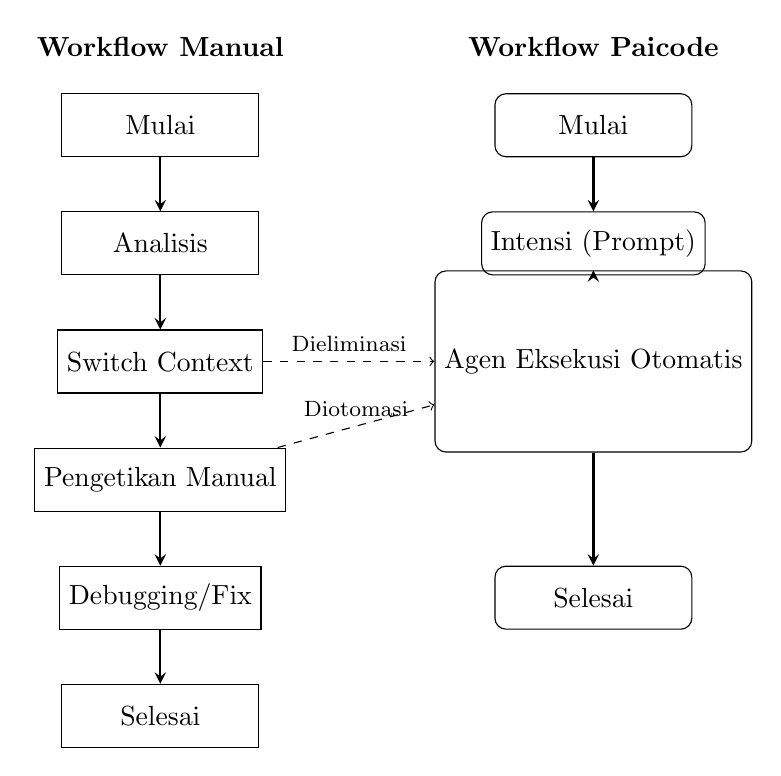
\begin{tikzpicture}[node distance=1.5cm, auto,
    manual/.style={rectangle, draw=black, minimum width=2.5cm, minimum height=0.8cm, text centered},
    agent/.style={rectangle, draw=black, minimum width=2.5cm, minimum height=0.8cm, text centered, rounded corners},
    arrow/.style={thick,->,>=stealth}
  ]
    % Manual Flow
    \node (m_start) [manual] {Mulai};
    \node (m_think) [manual, below of=m_start] {Analisis};
    \node (m_switch) [manual, below of=m_think] {Switch Context};
    \node (m_type) [manual, below of=m_switch] {Pengetikan Manual};
    \node (m_debug) [manual, below of=m_type] {Debugging/Fix};
    \node (m_end) [manual, below of=m_debug] {Selesai};
    
    \draw[arrow] (m_start) -- (m_think);
    \draw[arrow] (m_think) -- (m_switch);
    \draw[arrow] (m_switch) -- (m_type);
    \draw[arrow] (m_type) -- (m_debug);
    \draw[arrow] (m_debug) -- (m_end);
    
    % Agent Flow
    \node (a_start) [agent, right of=m_start, xshift=4cm] {Mulai};
    \node (a_intent) [agent, below of=a_start] {Intensi (Prompt)};
    \node (a_agent) [agent, below of=a_intent, minimum height=2.3cm] {Agen Eksekusi Otomatis};
    \node (a_end) [agent, below of=a_agent, yshift=-1.5cm] {Selesai};
    
    \draw[arrow] (a_start) -- (a_intent);
    \draw[arrow] (a_intent) -- (a_agent);
    \draw[arrow] (a_agent) -- (a_end);
    
    % Labels
    \node [above of=m_start, yshift=-0.5cm] {\textbf{Workflow Manual}};
    \node [above of=a_start, yshift=-0.5cm] {\textbf{Workflow Paicode}};
    
    % Annotation
    \draw [dashed, ->] (m_switch) -- node[above, font=\footnotesize] {Dieliminasi} (a_agent);
    \draw [dashed, ->] (m_type) -- node[above, font=\footnotesize] {Diotomasi} (a_agent);
    
  \end{tikzpicture}
  \caption{Perbandingan alur kerja Manual vs Paicode. Paicode mengeliminasi \textit{context switching} dan beban pengetikan.}
  \label{fig:workflow-comparison}
\end{figure}

\subsection{Keterbatasan Sistem}
Meskipun berhasil memenuhi tujuan utama, sistem masih memiliki keterbatasan:
\begin{enumerate}
    \item Kualitas kode sangat bergantung pada model LLM yang digunakan. Jika API sedang mengalami degradasi layanan, performa agen ikut menurun.
    \item Konteks jendela (\textit{context window}) terbatas. Untuk proyek skala besar dengan ratusan berkas, agen belum bisa "melihat" keseluruhan proyek sekaligus tanpa strategi \textit{retrieval augmented generation} (RAG) yang lebih canggih.
\end{enumerate}
